\documentclass[12pt, letterpaper]{article} % [Tamano de la fuente, Tamano del papel]

% Tamano de la pagina y margenes.
\usepackage[letterpaper,top=2cm,bottom=2cm,left=3cm,right=3cm,marginparwidth=1.75cm]{geometry}

% packages utiles
\usepackage{amsmath}
\usepackage[colorlinks=true, allcolors=black]{hyperref}
\usepackage{graphicx}
\graphicspath{{imagenes\}}} % Direccion de las imagenes
\usepackage{listings}
\usepackage[utf8]{inputenc}

% Tamano de la pagina y margenes.
\usepackage[left=3cm, 
    right=3cm,
    top=2cm,
    bottom=2cm]{geometry}

% packages utiles
\usepackage{amsmath}
\usepackage{graphicx}
\usepackage{float}
\usepackage{listings}
\usepackage[utf8]{inputenc}
\usepackage[spanish]{babel}
\usepackage{parskip}
\usepackage{hyperref}
\usepackage{fancyhdr}

% Portada
\begin{document}  
\thispagestyle{empty}
	
	\begin{figure}[h]
	        \minipage[t]{.5\textwidth}
		   	          
\includegraphics[height=4cm]{Img/Logo_UNAM.png}
			          
	        \endminipage
	\hfill
	        \minipage[t]{.2\textwidth}
		           	  
\includegraphics[height=4cm]{Img/Logo_Fi.jpg}
		  	          
		    \endminipage
	\end{figure}
	
    \begin{center}
    	\vspace{0.8cm}
    	\LARGE
	    UNIVERSIDAD NACIONAL
	    AUTÓNOMA DE MÉXICO
	
    	\vspace{0.6cm}
    	\LARGE
         {FACULTAD DE INGENIERÍA}
    	
    	\vspace{1 cm}	
    	\LARGE
    	\textbf{Proyecto Final - Base de Datos para un restaurante}
	   
	\vspace{1cm}
	\large
	INTEGRANTES DEL EQUIPO: DATA MATRIX Studios\\
	\vspace{.3cm}
	\large
	\textbf{Alvarez Saldaña Ariana Lizeth\\ López González Erick \\ R Alan }

	\vspace{1cm}
	\large
	PROFESOR \\
	\vspace{0.2cm}
	\large
	\textbf{Arreola Fernando} \\
	\vspace{1cm}
	\large	
	ASIGNATURA \\
	\vspace{.3cm}
	\large
	\textbf{Bases de Datos}
	
	\vspace{1cm}
    \large	
	FECHA DE ENTREGA \\
	\vspace{.3cm}
	\large
	\textbf{26 de Noviembre de 2023}
    \end{center}

\newpage

% Índice
\tableofcontents

\newpage
\section{Introduccion}

Este documento aborda la resolución de un problema relacionado con la creación de una base de datos para un restaurante que busca digitalizar sus operaciones. Para ello, se presenta un diseño, detallado más adelante en este documento, con el objetivo de cumplir con lo siguiente:

\begin{itemize}
    \item Almacenar información sobre:
        \begin{itemize}
            \item Empleados (Cocineros, Meseros y Administrativos).
            \item Dependientes económicos de los empleados.
            \item Platillos y bebidas.
            \item La Categoría de los platillos y bebidas.
            \item El contenido completo de una Orden
            \item Información del Cliente para elaborar su Factura de consumo.
        \end{itemize}
    
\end{itemize}

Además, se plantean los siguientes requerimientos específicos:
\begin{itemize}
    \item Mostrar, a partir del número de un empleado, la cantidad de órdenes registradas por el restaurante en el día, así como el total pagado por dichas órdenes.

    \item Visualizar una vista que detalle la información del platillo más vendido.

    \item Permitir la obtención de los nombres de los productos que no se encuentran disponibles.

    \item Mostrar una vista que contenga la información necesaria para simular una factura de una orden.

    \item Al proporcionar una fecha o un rango de fechas, obtener el total del número de ventas y el monto total de ventas en ese período de tiempo.
\end{itemize}

Estos objetivos y requerimientos guiarán el diseño y desarrollo de la base de datos del restaurante.


\newpage
%Análisis de la implementacion
\section{Plan de trabajo}
Para el proyecto, es necesario elaborar los siguientes productos:

\begin{itemize}
    \item La documentación pertiente.
    
    \item Los códigos fuente del Modelo Entidad Relación y Modelo Relacional.

    \item El script de creación de la base de datos y las tablas que almacenaran la información.

    \item El script para agregar información a las tablas.

    \item Los scripts de toda la programación a nivel de la base de datos.

    \item El código implementado para la etapa de presentación.

    \item La presentación para exponer el proyecto.

\end{itemize}

Dichas actividades se repartieron de la siguiente forma enter los integrantes:

\begin{itemize}
    \item Alvarez Saldaña Ariana Lizeth
        \begin{itemize}
            \item Elaboración del modelo relacional.
            \item Creación de los insert para las tablas creadas.
        \end{itemize}
    \item López González Erick
        \begin{itemize}
            \item Creación del modelo entidad relación.
            \item Creación del script de la base de datos y las tablas.
            \item Creación del scripts de programación a nivel BD (Trigger e índice).
            \item Creación del documento en Latex.
        \end{itemize}
    \item R Alan
        \begin{itemize}
            \item Creación del script que permita visualizar la inforación de un empleado por medio de una app.
        \end{itemize}
    
\end{itemize}

\newpage
%Explicacion del programa
\section{Diseño}

La primera parte de diseño consistió en el análisis del enunciado propuesto:

\begin{figure}[h]
    \centering
    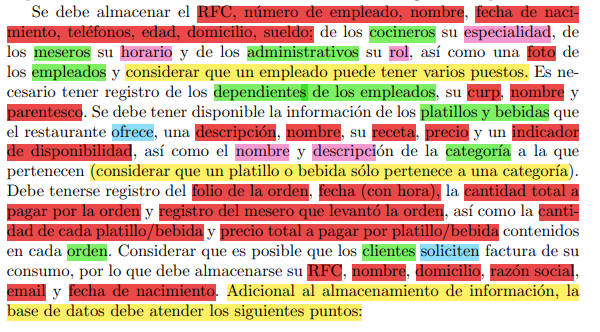
\includegraphics{Img/Analisis_Inicial.png}
    \caption{Identificación inicial. Donde: Entidad - Verde, Atributo - Rojo, Atributo de entidad derivada - Rosa, Relaciones - Azul, Consideraciones - Amarillo.}
\end{figure}

De esta primera parte, se lograrón identificar a las siguientes entidades:

\begin{itemize}
    \item Empleados (Cocineros, Meseros y Administrativos).
    \item Dependientes económicos de los empleados.
    \item Platillos y bebidas.
    \item La Categoría de los platillos y bebidas.
    \item La entidad Orden del cliente.
    \item Información del Cliente para elaborar su Factura de consumo.
\end{itemize}

Es entonces, y apoyados de las relaciones explícitas, relacionamos de la siguiente manera las entidades:

\begin{itemize}
    \item Empleados tiene Dependientes (1:m)
    
    Donde: Un empleado tiene niguno o varios dependientes, pero un dependiente solo se relaciona con un empleado.
    
    \item Mesero sirve una Orden (1:m)

    Donde: Un mesero sirve una o muchas ordenes, pero una orden solo puede ser serivida por un mesero.
    
    \item Orden genera una Factura (1:1)

    Donde: Una orden genera una factura y una factura es generada por una orden.
    
    \item Una Factura es solicitada por un Cliente (m:1)

    Donde: Un cliente solicta una o varias facturas, pero una factura solo es solicitada por un cliente.
    
    \item Una Orden contiene Alimentos (m:m)

    Donde: Una orden contiene uno o muchos alimentos y uno o varios alimetos pueden ser contenidos en una orden.
    
    \item Un Alimento pertenece a una Categoria (m:1)

    Donde: Una categoría puede tener varias alimentos, pero un alimento puede tener opcionalmente una categoría.
    
\end{itemize}

Igualmente, se analizarón algunos detalles en los atributos y entidades propuestas:

\begin{itemize}
    \item Entidad Dependiente:

    Para esta entidad se llegó a la conclusión de que es una entidad débil relacionada a la entidad empleado porque en la base de datos no nos interesa guardar dicha información a no ser que esté ligada a un empleado.

    \item Atributo teléfono de la entidad Empleado:

    Como el empleado puede guardar varios teléfonos, se tuvo que indicar que este atributo es multivaluado.

    \item Atributo total a pagar de la entidad Orden:

    Este atributo es un total a pagar que se calculará para mostrar en la factura, por lo que se indica que es del tipo derivado.

    \item Atributos ap Mat (apellido Materno) de todas la entidades que lo contienen:

    Finalmente, una persona puede o no tener un seguno apellido, por ello es necesario indicar que es opcional.

    \item Atributo cantidad platillo en la relación orden y alimento:

    Como nos interesa saber en cada orden cuantos platillo se pidieron, fue necesario integrar el atributo pertinente para llevar el registro y utilizarlo para el total a pagar.

\end{itemize}

\newpage
Finalmnete, el resultado de este análisis es el siguiente modelo:

\begin{figure}[h]
    \centering
    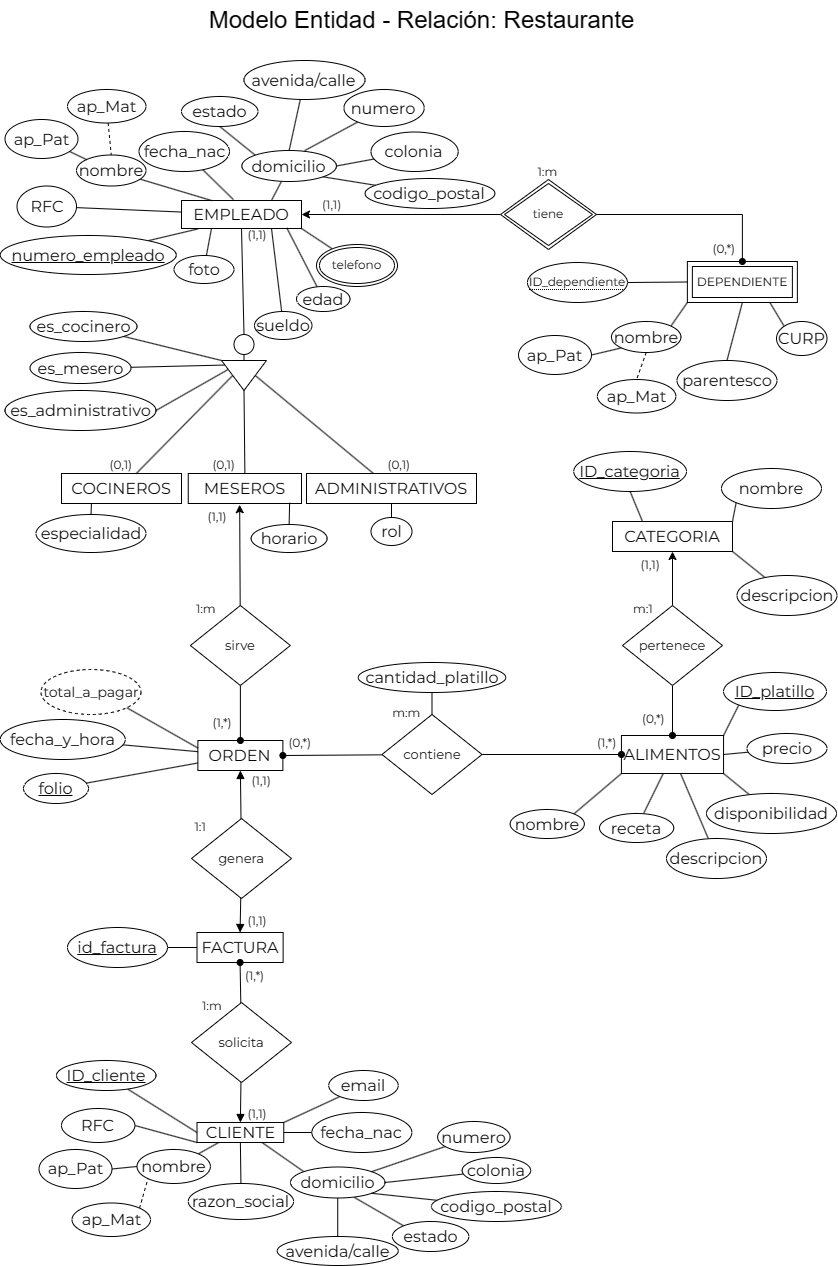
\includegraphics[scale=0.38]{Img/MER-Restaurante.png}
    \caption{Versión final del modelo.}
\end{figure}

\newpage
\section{Implementación}
Para la implementación de las tablas generadas en el modelo relacional, se codificó lo siguiente:

\begin{lstlisting}[language=SQL, caption=Creación de las tablas que almacenarán la información.]

-- @Autor: DataMatrix Studios
-- @Fecha creacion:  2023
-- @Descripcion: Creacion de las tablas para la BD de un restaurante.

-- Creacion de la base de datos
-- create database Restaurate;
-- \c Restaurate

--
-- ENTIDAD EMPLEADO
--

create table EMPLEADO
(
	Numero_empleado numeric(4, 0) PRIMARY KEY,
	RFC varchar(13) not null,
	Nombre_empleado varchar(50) not null,
	Apellido_paterno varchar(50) not  null,
	Apellido_materno varchar(50) null,
	Fecha_nacimiento Date not null,
	Edad numeric(3, 0) not null,
	Sueldo numeric(8, 2) not null,
	Foto bytea not null,
	-- Domicilio
	Estado varchar(50) not null,
	Avenida_calle varchar(50) not null,
	Numero_exterior_vivienda numeric(5, 0) null,
	Colonia varchar(50) not null,
	Codigo_postal numeric(6, 0) not null,
	-- Rol del empleado
	Es_cocinero bit null,
	Es_mesero bit null,
	Es_administrativo bit null
);

--
-- ATRIBUTO MULTIVALUADO DE EMPLEADO - TELEFONO
--

create table EMPLEADO_TELEFONO
(
	Numero_empleado numeric(4, 0),
	Telefono_Id numeric(10, 0),
	constraint EMPLEADO_TELEFONO_PK PRIMARY KEY(Numero_empleado,
    Telefono_Id)
);

--
-- ENTIDAD COCINERO - TIPO DE EMPLEADO
--

create table COCINERO
(
	Numero_empleado_cocinero numeric(4, 0) PRIMARY KEY,
	Especialdad varchar(50),
	constraint Numero_empleado_cocinero_Fk FOREIGN KEY
    (Numero_empleado_cocinero) references EMPLEADO(Numero_empleado)
);

--
-- ENTIDAD MESERO - TIPO DE EMPLEADO
--

create table MESERO
(
	Numero_empleado_mesero numeric(4, 0) PRIMARY KEY,
	Horario_descripcion varchar(500) not null,
	constraint Numero_empleado_mesero_Fk
    FOREIGN KEY (Numero_empleado_mesero)
    references EMPLEADO(Numero_empleado)
);

--
-- ENTIDAD ADMINISTRATIVO - TIPO DE EMPLEADO
--

create table ADMINISTRATIVO
(
	Numero_empleado_administrativo numeric(4, 0) PRIMARY KEY,
	Rol varchar(50) not null,
	constraint Numero_empleado_administrativo_Fk FOREIGN KEY
    (Numero_empleado_administrativo) references EMPLEADO(Numero_empleado)
);

--
-- ENTIDAD DEPENDIENTE - ENTIDAD DEBIL DE EMPLEADO
--

create table DEPENDIENTE
(
	ID_dependiente numeric(10, 0) not null,
	Numero_empleado numeric(4, 0) not null,
	Curp varchar(13) not null,
	Nombre_dependiente varchar(50) not null,
	Apellido_paterno varchar(50) not null,
	Apellido_materno varchar(50) null,
	Parentesco varchar(50) not null,
	constraint dependiente_pk PRIMARY KEY(ID_dependiente,
    Numero_empleado), constraint Numero_empleado_Fk
    FOREIGN KEY (Numero_empleado)
    references EMPLEADO(Numero_empleado)
);

--
-- ENTIDAD CLIENTE
--

create table CLIENTE
(
	ID_cliente numeric(10, 0) PRIMARY KEY,
	RFC_cliente varchar(13) not null,
	Nombre_cliente varchar(50) not null,
	Apellido_paterno varchar(50) not null,
	Apellido_materno varchar(50) null,
	Fecha_nacimiento Date not null,
	Razon_social varchar(500) not null,
	Email varchar(200) not null,
	-- Domicilio
	Estado varchar(50) not null,
	Avenida_calle varchar(50) not null,
 	Numero_exterior_vivienda numeric(5, 0) not null,
	Colonia varchar(50) not null,
	Codigo_postal numeric(6, 0) not null
);

--
-- ENTIDAD FACTURA
--

create table FACTURA
(
	ID_factura numeric(10, 0) PRIMARY KEY,
	ID_cliente numeric(10, 0) not null,
	constraint ID_cliente_fk FOREIGN KEY (ID_cliente)
    references CLIENTE(ID_cliente)
);

--
-- ENITDAD ORDEN
--

create table ORDEN
(
	Folio_orden varchar(14) PRIMARY KEY,
	Fecha_orden date not null,
	Total_a_pagar numeric(12, 2) not null,
	Mesero_atendio numeric(4, 0) not null,
	ID_factura numeric(10, 0) not null,
	constraint Mesero_atendio_fk FOREIGN KEY
    (Mesero_atendio) references MESERO(Numero_empleado_mesero),
	constraint ID_factura_fk FOREIGN KEY (ID_factura)
    references FACTURA(ID_factura),
	constraint chk_folio_orden check (Folio_orden = 'ORD-%')
);

--
-- ENTIDAD CATEGORIA
--

create table CATEGORIA
(
	ID_Categoria numeric(3, 0) PRIMARY KEY,
	Nombre_categoria varchar(100) not null,
	Descripcion_categoria varchar(500) not null
);

--
-- ENTIDAD ALIMENTOS (PLATILLO Y BEBIDA)
--

create table ALIMENTOS
(
	ID_ALIMENTO numeric(6, 0) PRIMARY KEY,
	Nombre_platillo varchar(100) not null,
	Receta_platillo varchar(1000) not null,
	Descripcion_platillo varchar(500) not null,
	Disponibilidad_platillo varchar(10) not null,
	Precio_platillo numeric(10, 2) not null,
	ID_Categoria numeric(3, 0) not null,
	constraint ID_Categoria_Fk FOREIGN KEY (ID_Categoria)
 references CATEGORIA(ID_Categoria)
);

--
-- ENITDAD RELACION M:M - RELACION ENTRE ORDEN Y PLATILLO
--

create table ORDEN_CONTIENE_PLATILLO
(
	ID_ALIMENTO numeric(6, 0) not null,
	Folio_orden varchar(14) not null,
	Cantidad_platillo numeric(5, 0) not null,
	constraint ID_ALIMENTO_Folio_orden_pk PRIMARY KEY
    (ID_ALIMENTO, Folio_orden),
	constraint ID_ALIMENTO_Fk FOREIGN KEY (ID_ALIMENTO)
    references ALIMENTOS(ID_ALIMENTO),
	constraint Folio_orden_Fk FOREIGN KEY (Folio_orden)
    references ORDEN(Folio_orden)

);
\end{lstlisting}

Este script (s-01-creacion-tablas.sql) tiene que ser el primer ejecutado pues creará las tablas pertinente, donde igualmente, en caso de no tener la base creada aún, se pueden quitar los comentarios de las líneas abajo del comentario "Creación de la base de datos" crear la BD.

A continuación, se necesitan ejecutar los triggers e índices que coexistiran en la base de datos.

Para el índice, se propuso colocar uno en la tabla Empleado y otro en la tabla Cliente:

\begin{lstlisting}[language=SQL, caption=Creación de índece para empleado y cliente.]
-- @Autor: DataMatrix Studios
-- @Fecha creacion:  2023
-- @Descripcion: Crear al menos, un indice, del tipo
--                que se prefiera y donde se prefiera.

--
-- Indice para Empleado
--

CREATE INDEX rfc_empleado_idx ON EMPLEADO(RFC);

--
-- Indice para Cliente
--

CREATE INDEX rfc_cliente_idx ON CLIENTE(RFC_cliente);
\end{lstlisting}

La elección de estos dos índices se debió a que podemos facilitar la búsqueda para los empleados y clientes a través de su RFC, un dato que se otorga comúnmente para generar la factura del consumo y que para los empleados se puede utilizar igualmente para facilitar su búsqueda.

Para el trigger se plantea lo siguiente:

\begin{lstlisting}[language=SQL, caption=Creación del trigger.]
--@Autor: DataMatrix Studios
--@Fecha creacion:  2023
--@Descripcion: Se busca suplir lo siguiente: Cada que se agregue
--                  un producto a la orden, debe actualizarse los
--                  totales (por producto y venta), asi como validar
--                  que el producto este disponible


CREATE OR REPLACE FUNCTION actualizar_totales_y_validar_producto() 
RETURNS TRIGGER AS $$
DECLARE
    total_por_producto NUMERIC(12, 2);
    total_venta NUMERIC(12, 2);
BEGIN
    -- Validar si el producto esta disponible
    IF NOT EXISTS (
        SELECT 1
        FROM ALIMENTOS
        WHERE ID_ALIMENTO = NEW.ID_ALIMENTO AND Disponibilidad_platillo = 'Disponible'
    ) THEN
        RAISE EXCEPTION 'El producto no se encuentra disponible';
    END IF;

    -- Calcular el total por producto (cantidad * precio)
    total_por_producto := NEW.Cantidad_platillo * (
        SELECT Precio_platillo FROM ALIMENTOS WHERE ID_ALIMENTO = NEW.ID_ALIMENTO
    );

    -- Actualizar el total por producto en ORDEN_CONTIENE_PLATILLO
    UPDATE ORDEN_CONTIENE_PLATILLO 
    SET total_por_producto = total_por_producto 
    WHERE ID_ALIMENTO = NEW.ID_ALIMENTO AND Folio_orden = NEW.Folio_orden;

    -- Calcular el total de la venta (sumar los totales por producto para la orden)
    total_venta := (
        SELECT SUM(total_por_producto) FROM ORDEN_CONTIENE_PLATILLO WHERE Folio_orden = NEW.Folio_orden
    );

    -- Actualizar el total de la venta en la tabla ORDEN
    UPDATE ORDEN SET Total_a_pagar = total_venta WHERE Folio_orden = NEW.Folio_orden;

    RETURN NEW;
END;
$$ LANGUAGE plpgsql;

CREATE TRIGGER actualizacion_totales_orden
AFTER INSERT ON ORDEN_CONTIENE_PLATILLO
FOR EACH ROW
EXECUTE FUNCTION actualizar_totales_y_validar_producto();
\end{lstlisting}

\newpage
%Presentación
\section{Presentación}
Descripcin de lo que hace la modalidad seleccionada como forma de conexión hacia la base de datos.

\newpage
%Conclusiones
\section{Conclusiones}
\textbf{Alvarez Saldaña Ariana Lizeth:}
El proyecto tuvo sus complicaciones, sin embargo se logro obtener una comprension con respecto a la base de datos solicitado. Especificando algunas dificultades, fueron el encontrar un software adecuado para la elaboracion de las tablas y modelos, ademas de la programacion de la base de datos, esto por las diferentes estr\\ \\

\vspace{0.5cm}

\textbf{López González Erick:} \\ \\
En la realización del proyecto, el problema más complicado fue la organización a nivel de equipo. Durante el desarrollo del proyecto, se inicio de forma correcta y se logró tener la propuesta del modelo entidad relación en la segunda semana del mes, pero es a partir de ello que la comunicación en el equipo se corto, esto aunado a que un miembro del equipo decidió retirarse, aumento la carga de trabajo para cada integrante y terminó por desembocar en la entrega incompleta del proyecto. Igualmente, a nivel personal se tuvieron complicaciones a la hora de asignarle tiempo  al proyecto a causa de la carga de trabajo en cuanto a tareas, prácticas, proyectos y examenes que trae consigo el fin de semestre.

Hablando sobre el desarrollo del mismo, mi principal reto fue la solución a los problemas relacionados con la programación a nivel de Base de Datos, para intentar su solución se necesito la búsqueda de ejemplos de aplicación a través de la web, así como del apoyo del material brindado por el laboratorio de la asignatura. Si bien el material me ayudó mucho, fue complicado tener que estar manejando postgres a causa de que mi experiencia obtenida en el laboratorio se realizó en Oracle BD.

Finalmente, en cuanto aciertos, considero que el diseño inicial de la base de datos a través del modelo entidad relación, si bien no fue el más óptimo, sirvió como solución inicial para la parte de almacenar los datos propuestos.

\vspace{0.5cm}

\textbf{R Alan :}  \\ \\
Conclusión

\end{document}
